\documentclass[12pt, a4paper]{article}
\usepackage[english]{babel}
\usepackage[margin=1.75cm]{geometry}
\usepackage{float}
\usepackage{graphicx}
\usepackage{hyperref}

\renewcommand{\familydefault}{\sfdefault}


\begin{document}
    \title{
        
\includegraphics[width=0.2\textwidth]{assets/logo.png}\\
        [0.5cm]CucinAssistant: How to\\
        \large updated to version \emph{8 (Banana)}
    }
    \author{Gianluca Parri}
    \date{\today}
    \maketitle



    \tableofcontents
    \vfill
    \noindent For errors and suggestions you can write at
    \href{mailto:info@cucinassistant.com}{\mbox{info@cucinassistant.com}}.



    \section{News}
    
    Since the last version (\emph{7 (Ciliegia)}), CucinAssistant had the
    following changes:

    \begin{itemize}
        \item Menu structure customizable (\ref{menus})
        \item Changed all the icons
    \end{itemize}

    \begin{figure}[H]
        \centering
        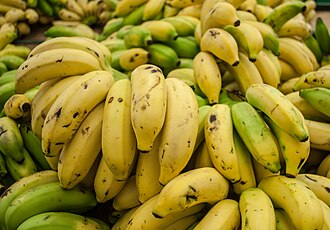
\includegraphics[width=0.45\textwidth]{assets/banane.jpg}
		\caption{\emph{Banane}. Photo from \href{https://commons.wikimedia.org\
            /wiki/File:Cavendish_banana_from_Maracaibo.jpg}{here}.}
    \end{figure}


    \section{Introduction}

    \subsection{Language setting}

    You can change CucinAssistant's language anytime by clicking on the icon at
    the logo's left, on the navigation bar on the top of every page.

    \begin{figure}[H]
        \centering
        
\includegraphics[width=0.45\textwidth]{assets/nav.png}
    \end{figure}

    \subsection{Sign up and sign in}

    If you already have an account you can fill in the form on the sign in page
    straight away; on the other hand, you can sign up using the button below.

    If you have an account, but you've lost your username and/or your password,
    you can use the \emph{Forgot password} button, that will send you an
    email containing both the username and a link to reset your password.

    \begin{figure}[H]
        \centering
        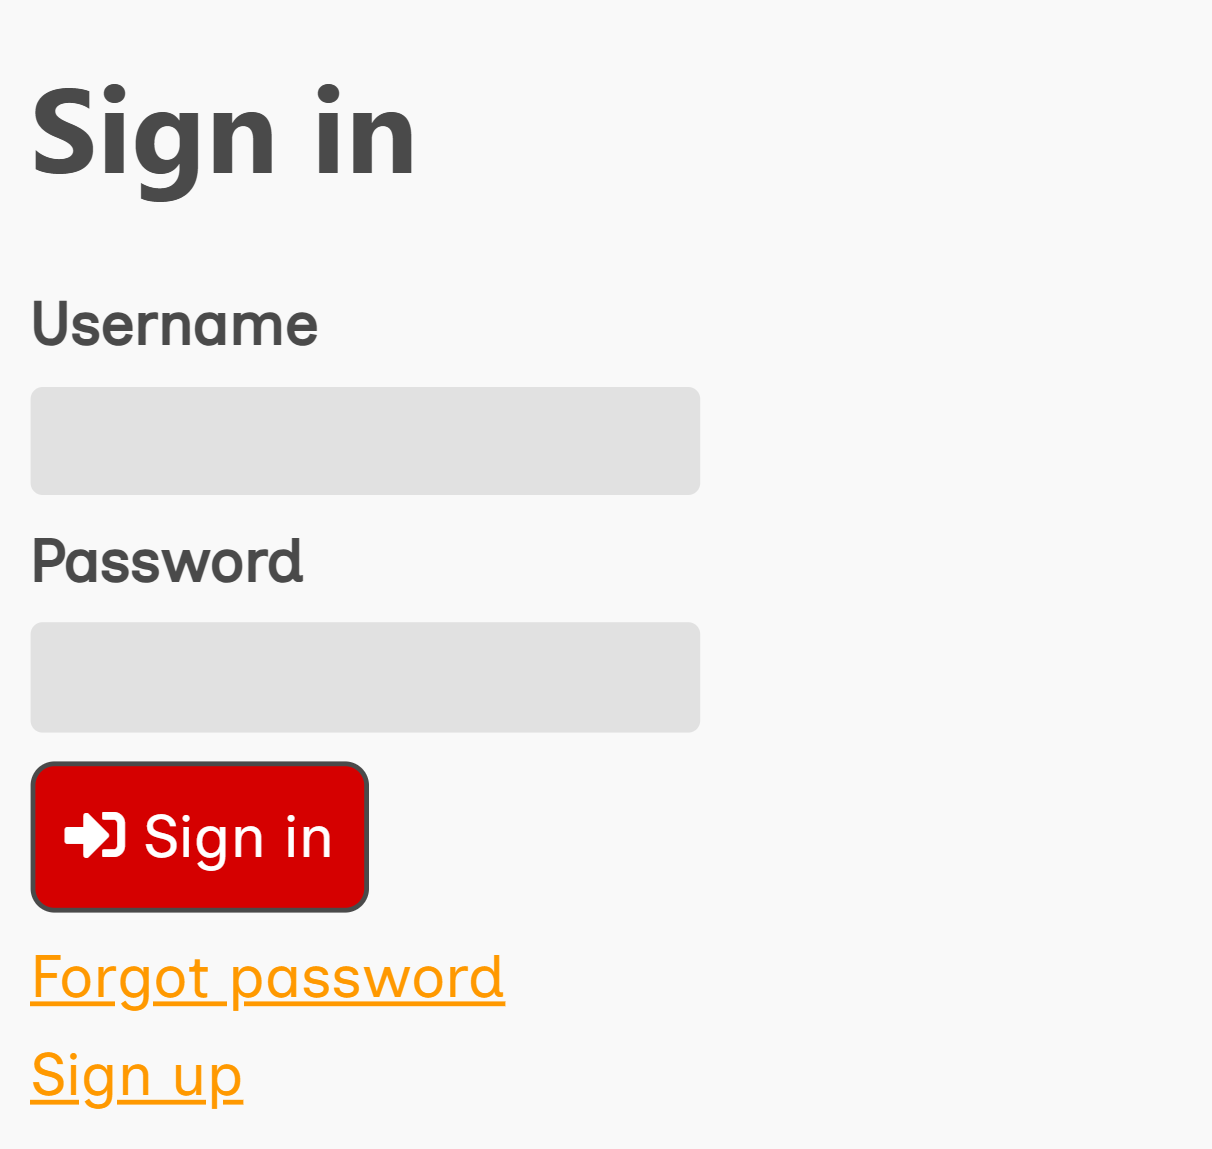
\includegraphics[width=0.45\textwidth]{assets/en/signin.png}
    \end{figure}

    Once signed in, you'll gain access to the \emph{homepage}.

    \begin{figure}[H]
        \centering
        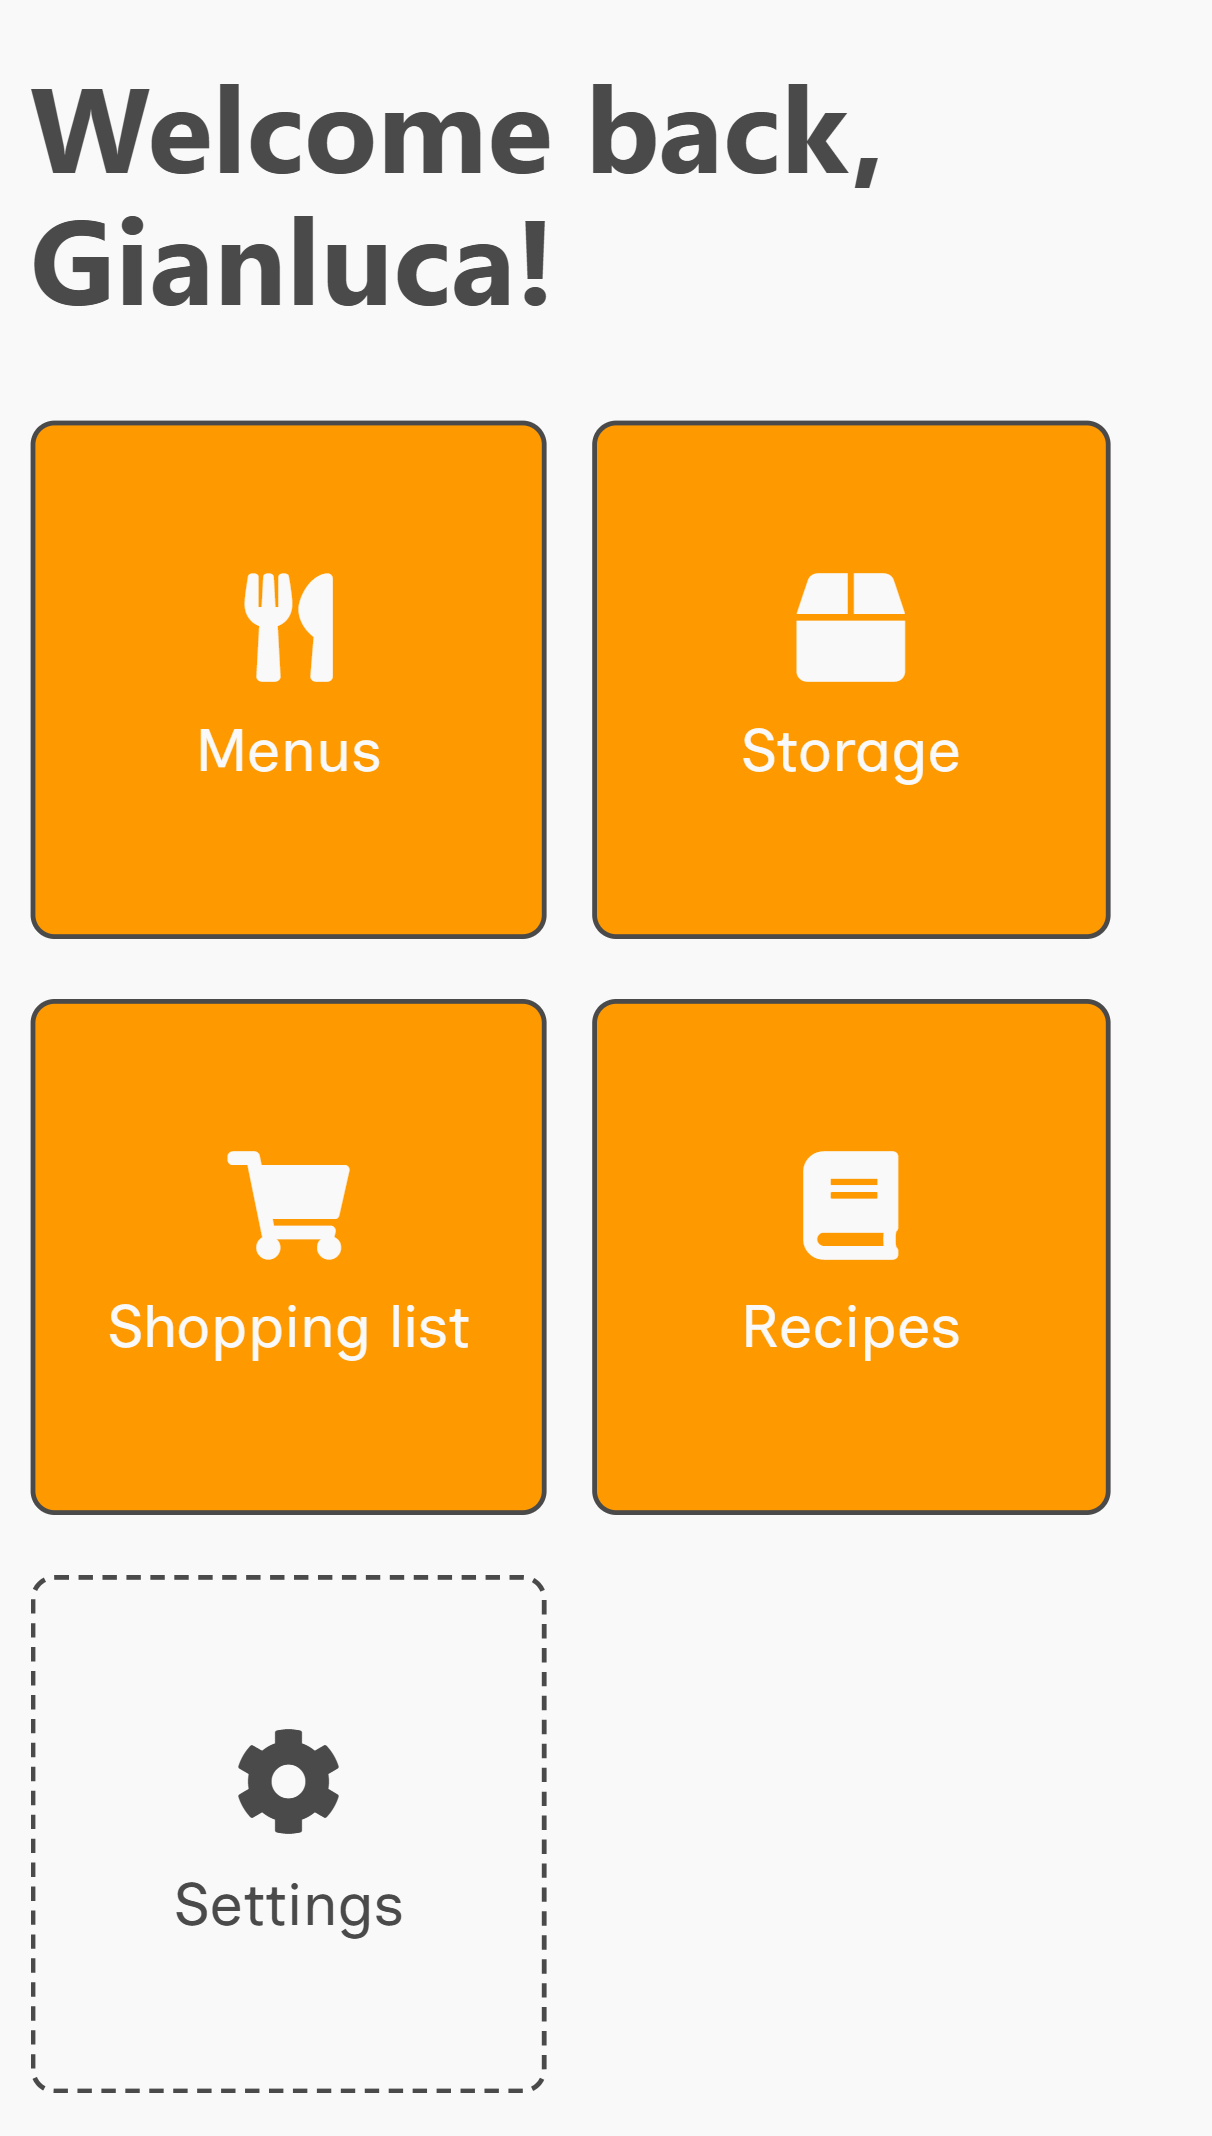
\includegraphics[width=0.45\textwidth]{assets/en/home.png}
    \end{figure}

    \subsection{Settings}

    The settings page contains a button to sign out, some buttons to change
    your personal data (username, email and password), your email preferences
    (language and newsletter consent), and a button to permanently
    delete your account.

    \begin{figure}[H]
        \centering
        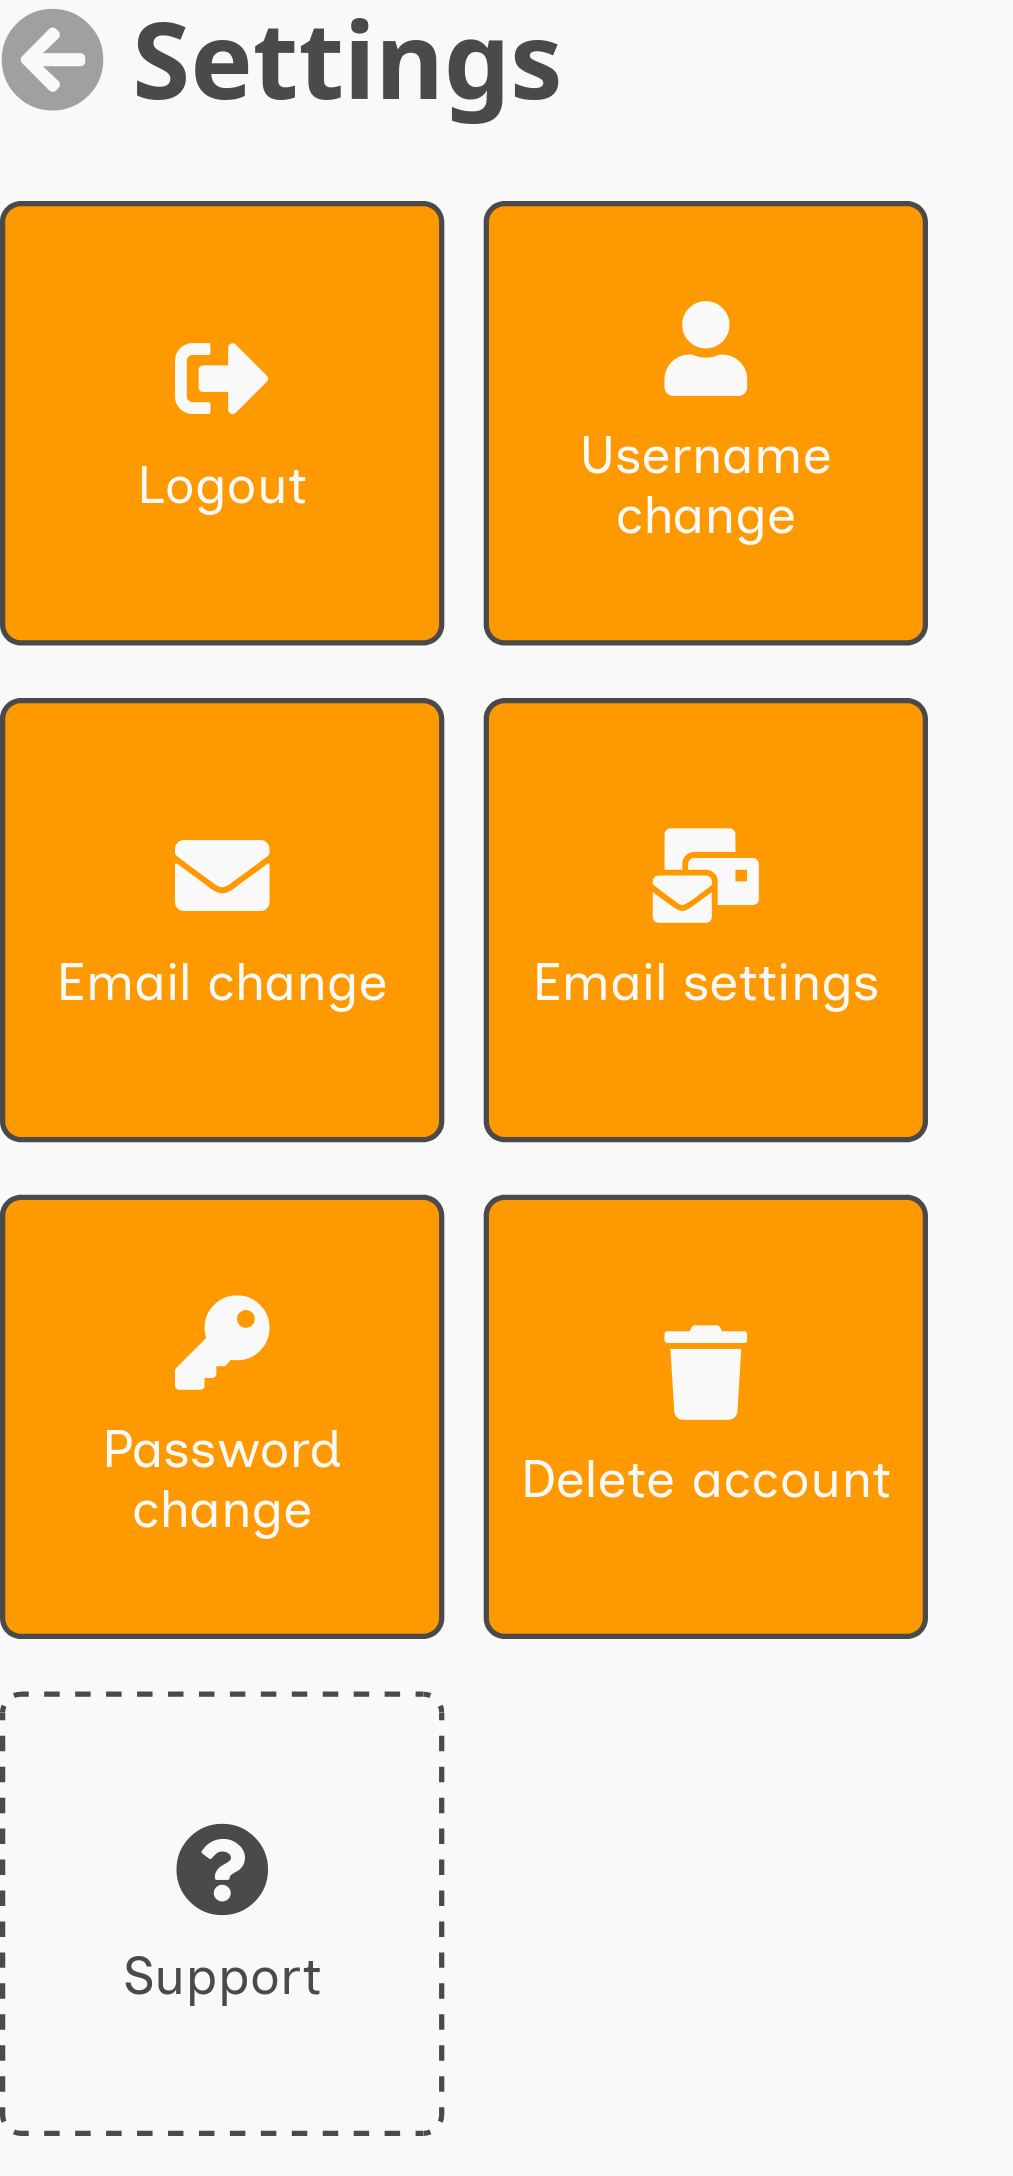
\includegraphics[width=0.45\textwidth]{assets/en/settings.png}
    \end{figure}


    \section{Menus} \label{menus}

    \subsection{Creation}

    By clicking the \emph{New menu} button, you will be able to create a new
    menu, specifiying which days are included and the number of meals per day.

    \begin{figure}[H]
        \centering
        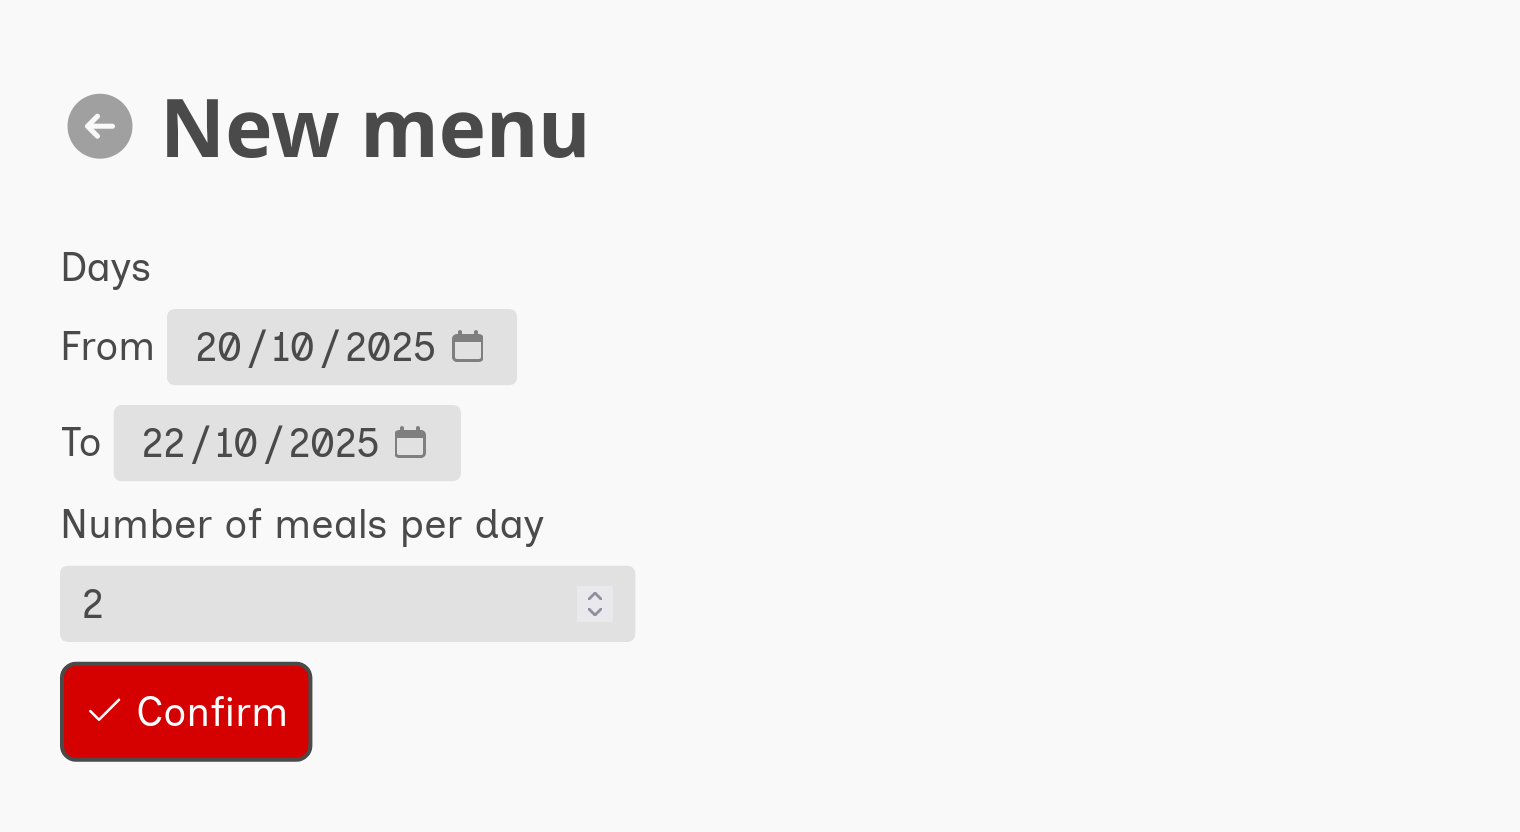
\includegraphics[width=0.45\textwidth]{assets/en/menu_new.png}
    \end{figure}

    \subsection{Editing}

    To edit a menu, you can click the \emph{Edit} button.

    Once clicked, you will be able to edit the menu's name and delete it;
    furthermore, you'll see a series of buttons used to edit each day.

    \begin{figure}[H]
        \centering
        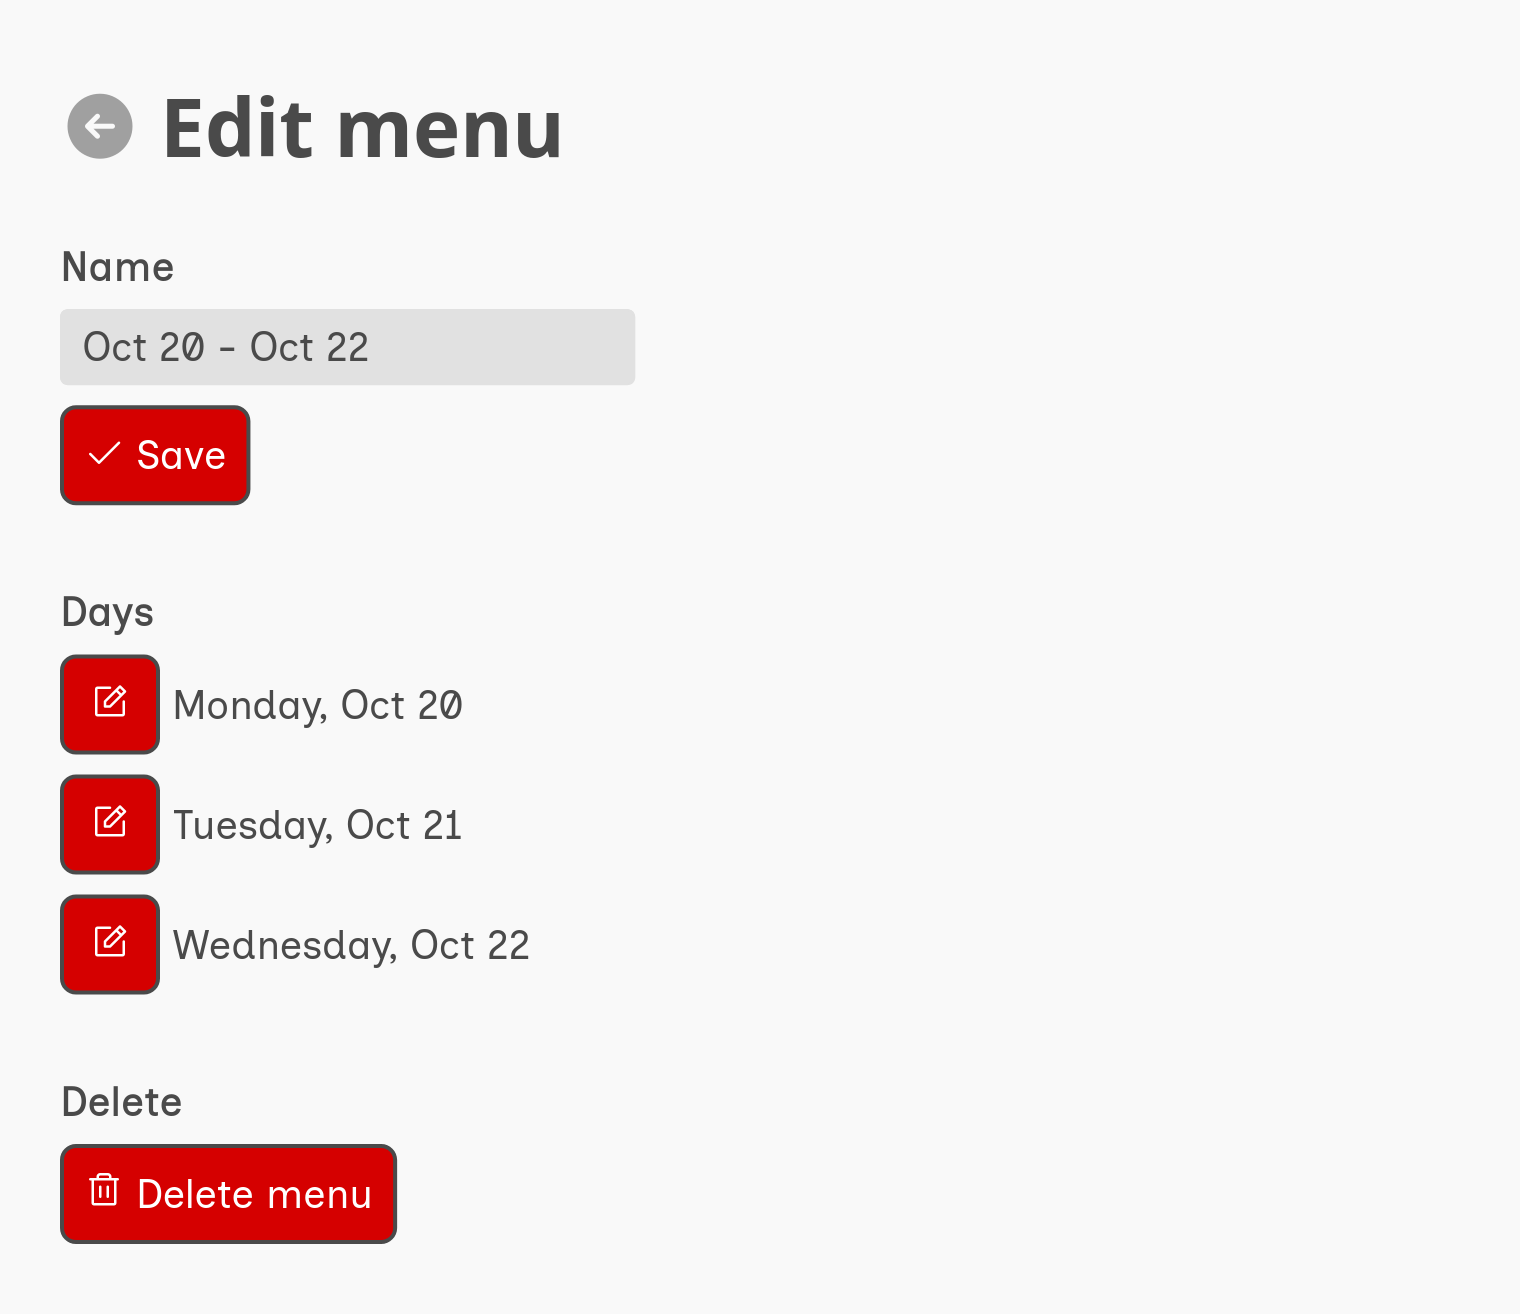
\includegraphics[width=0.45\textwidth]{assets/en/menu_edit.png}
    \end{figure}

    In the \emph{Edit day} page you will be able to change the day's name, or
    change its meals, adding or removing them if you need.

    \begin{figure}[H]
        \centering
        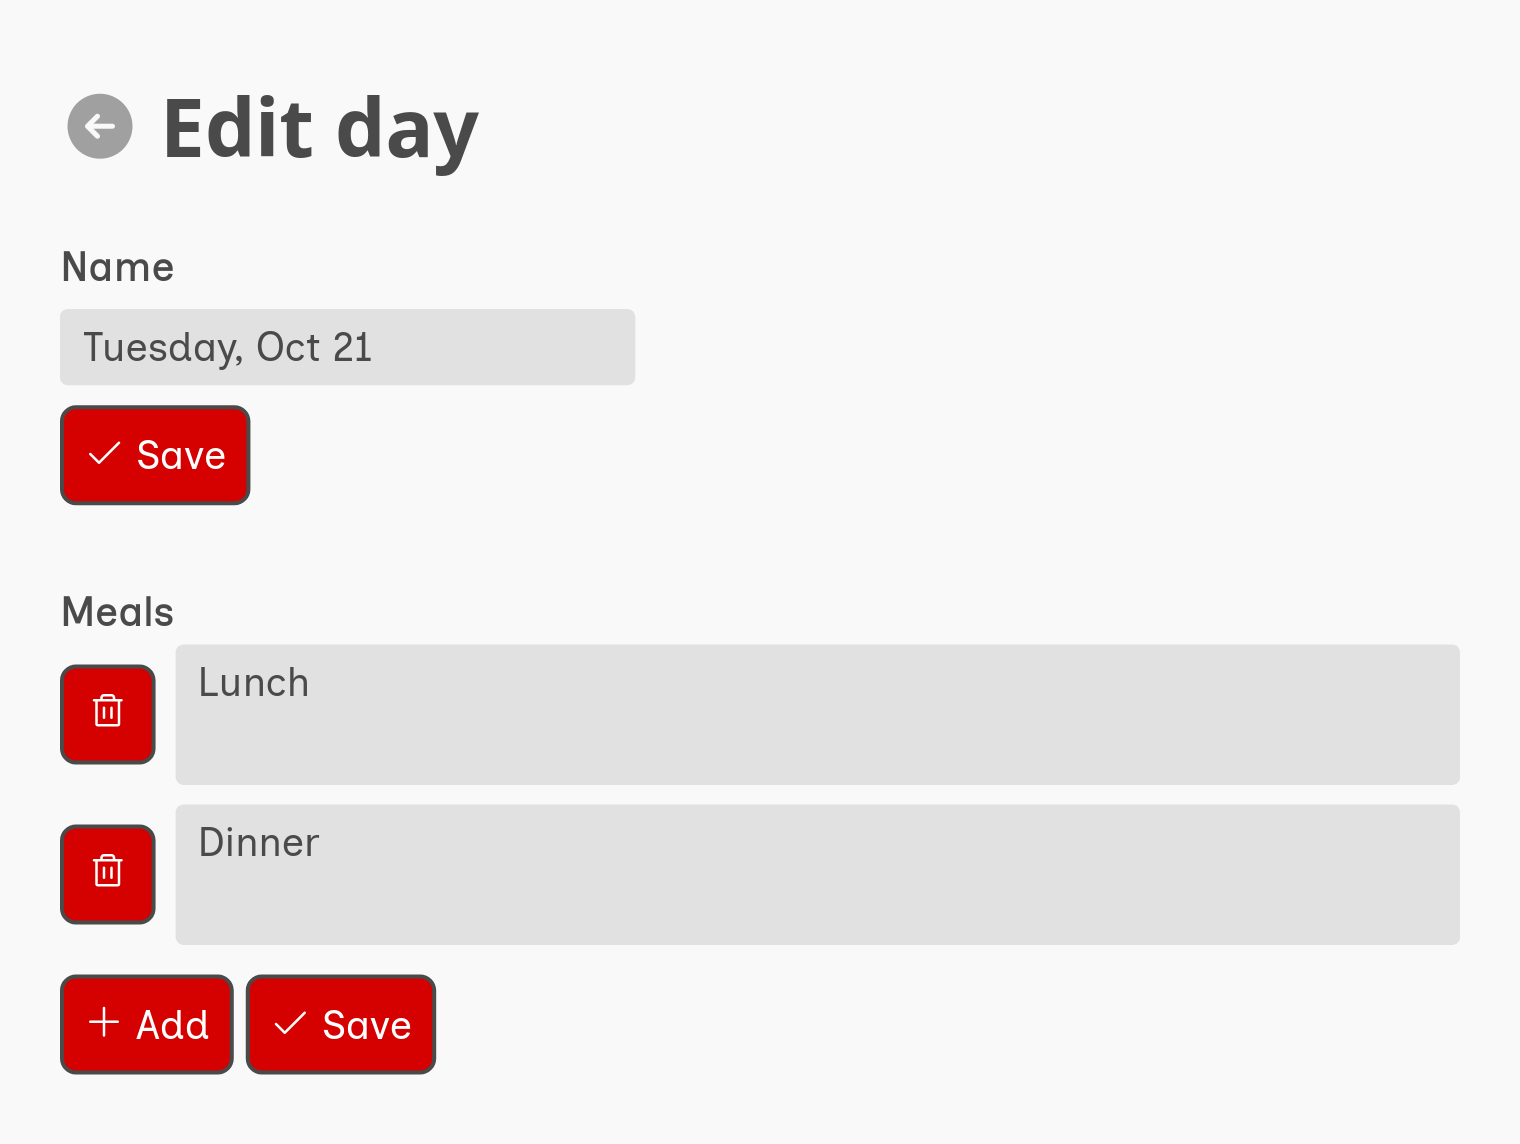
\includegraphics[width=0.45\textwidth]{assets/en/menu_day.png}
    \end{figure}



    \section{Storage}

    Inside the storage, you can save articles, with a name, an expiration date
    (optional) and a quantity (integer or decimal; optional).

	\subsection{Sections}

    The articles can be grouped into sections, which you will any time you open
    the \emph{Storage}.

    \begin{figure}[H]
        \centering
        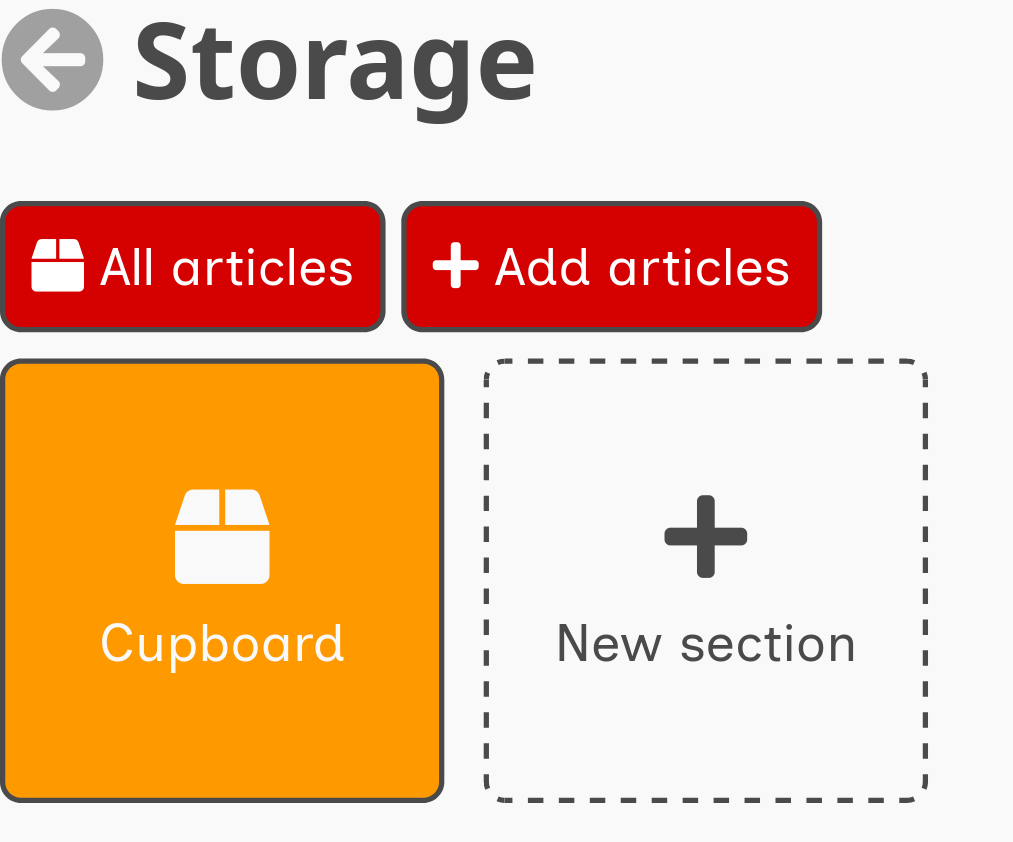
\includegraphics[width=0.45\textwidth]{assets/en/storage.png}
    \end{figure}

    You can create new sections with the button in the dashboard; to edit or
    delete one of them you have to open it and click the \emph{Edit section}
    button.

    \subsection{Articles}

    You can see the articles of each section (or all of them) by opening it.
    If you want, you can search for a name.

    Articles are ordered by their expiration date; the expired ones will have a
    red band on the left, instead of the orange one.

    \begin{figure}[H]
        \centering
        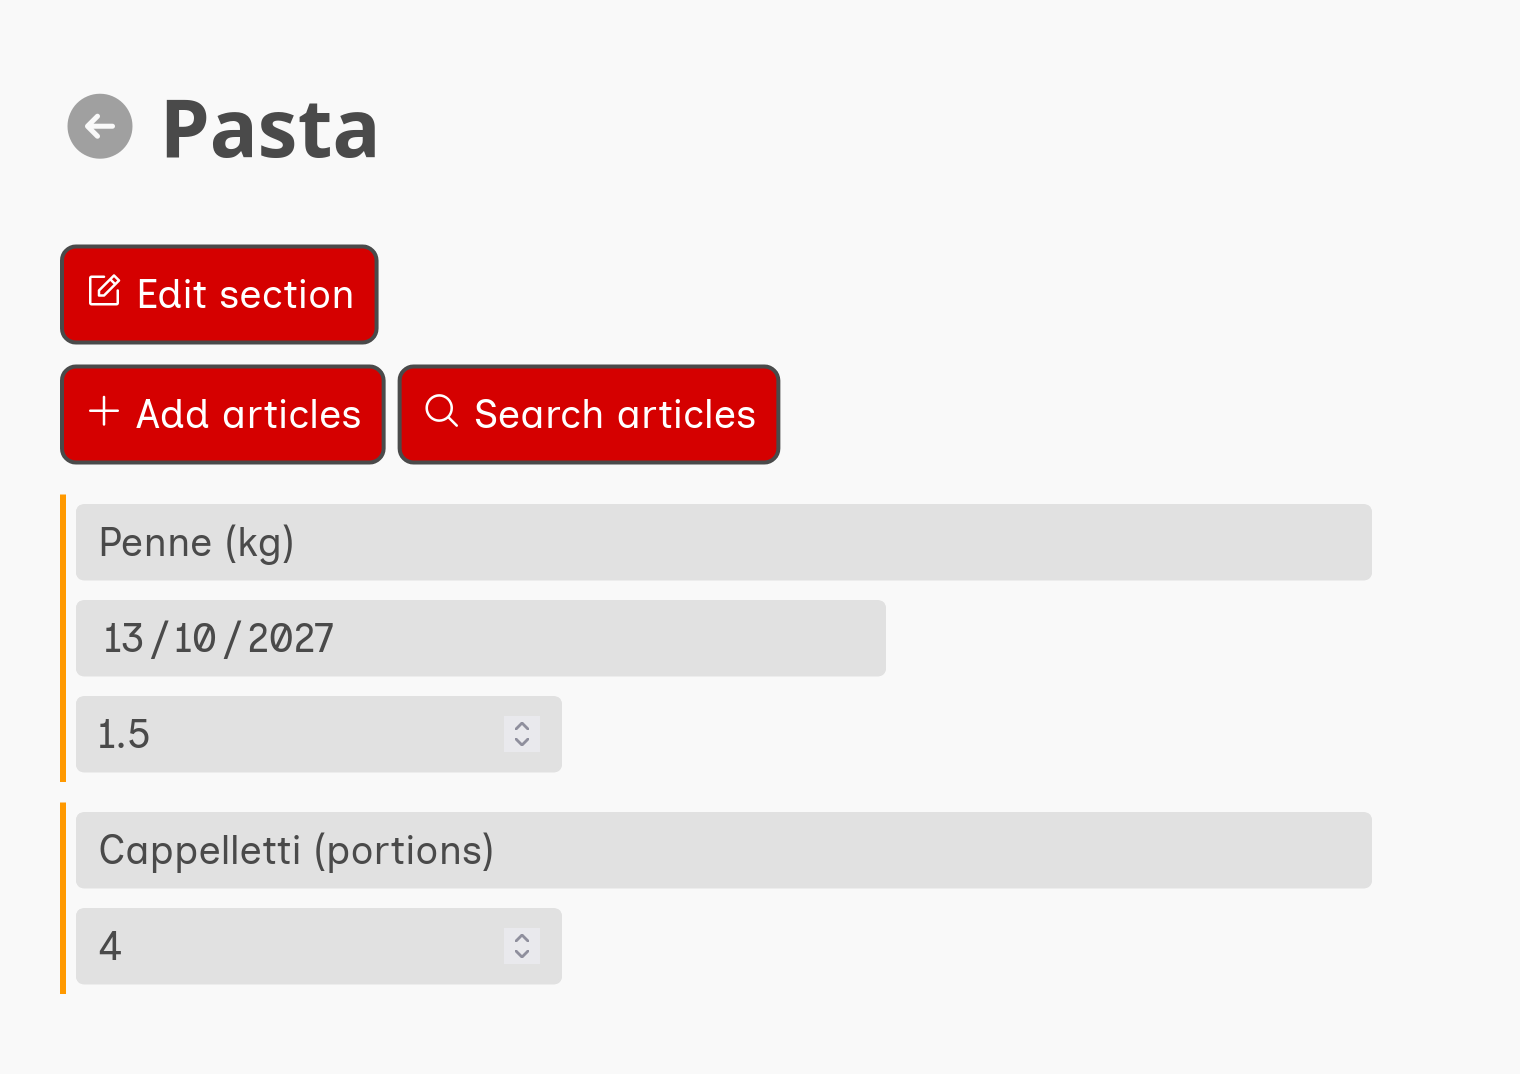
\includegraphics[width=0.45\textwidth]{assets/en/articles.png}
    \end{figure}

    You can add articles both from inside a section and outside a section; in
    the latter case, for each article to add you'll have to specify in which
    section to save it.

    An article is identified by its name and expiration date, so if you'll try
    to add an article that you already have in storage, CucinAssistant will sum
    the quantities, and not create duplicates. 

    \subsection{Articles editing}

    By clicking on an article, you'll see it alone with some arrows (used for
    scrolling between articles) and a \emph{Delete} button.

    Once you've changed some data, the buttons will be replaced with a
    \emph{Save} and a \emph{Discard} button, used to confirm your changes.
    If you change the section, the article will be moved.

    When changing an expiration date, the order of the articles may change: in
    this case, you'll be redirected at the list view.

    \begin{figure}[H]
        \centering
        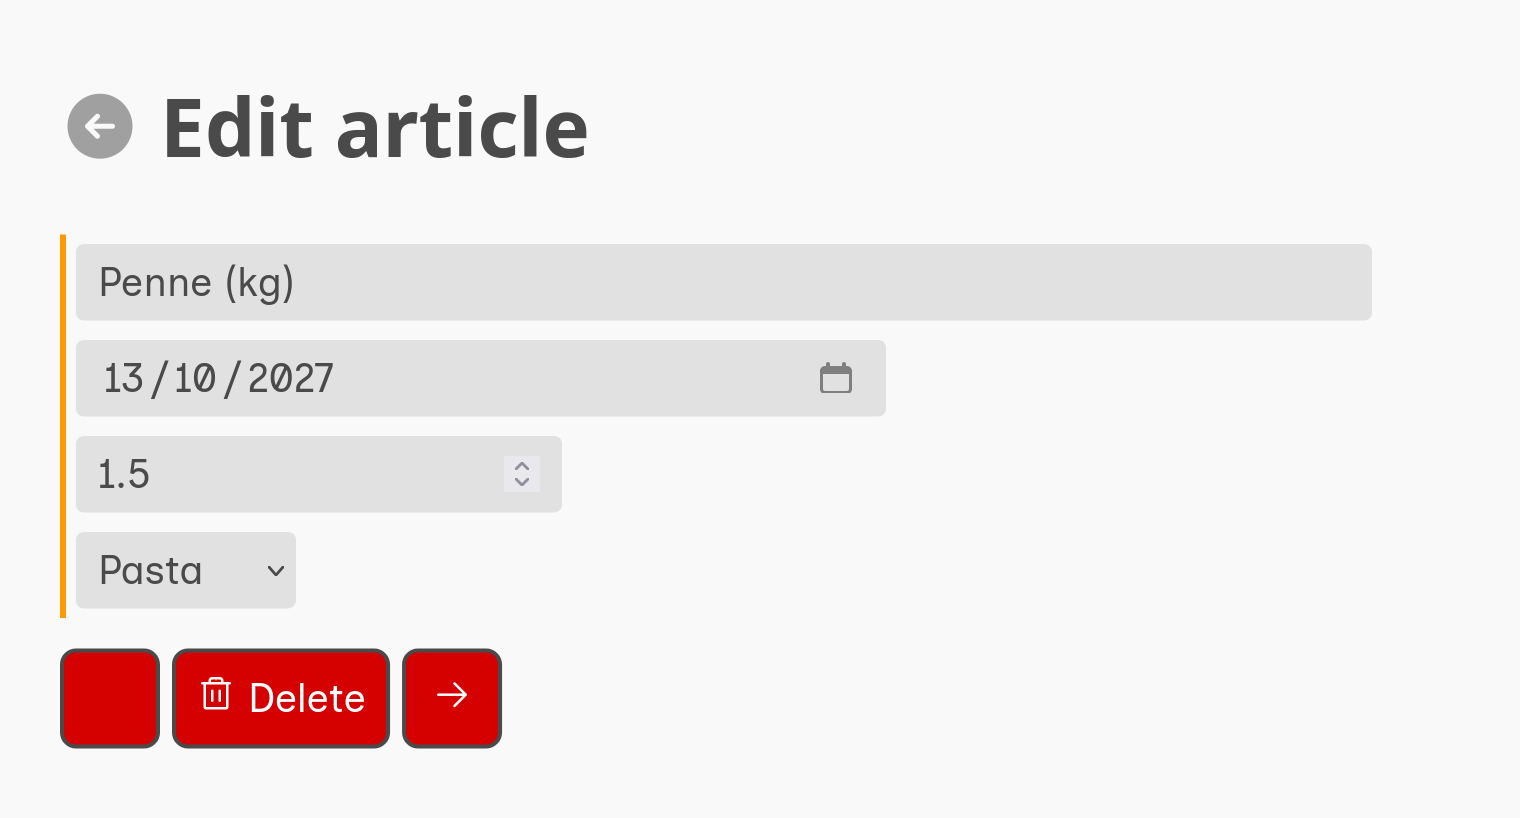
\includegraphics[width=0.45\textwidth]{assets/en/article.png}
    \end{figure}



    \section{Shopping List}

    \subsection{Overview}

    It's just... a list of things to buy.

    \begin{figure}[H]
        \centering
        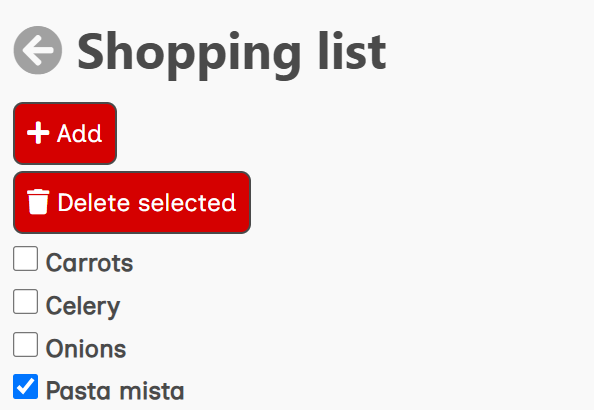
\includegraphics[width=0.45\textwidth]{assets/en/shopping_list.png}
    \end{figure}

    When you click the checkbox at the left of the entry, it will become
    checked, but will remain on the list; to remove all the checked ones you'll
    have to click the \emph{Delete selected} button.

    To add new items you can click the \emph{Add} button; to edit one of them,
    just click on its name.



    \section{Recipes}

    A recipe has a name (the only compulsory field), and a rating (0.5 to 5.0
    stars), some ingredients, some directions and some notes.

    \subsection{Overview}

    When you click the \emph{Recipes} button you'll see all your recipes and a
    button to create new ones.

    \begin{figure}[H]
        \centering
        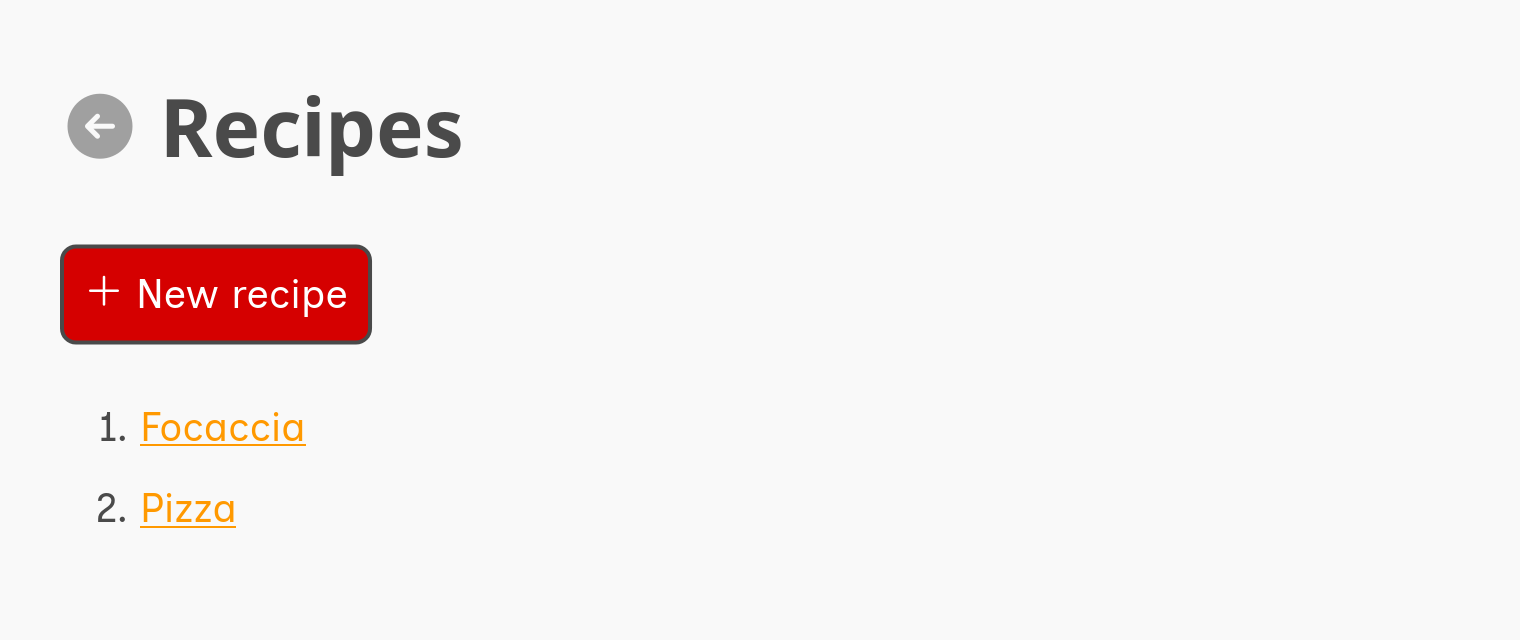
\includegraphics[width=0.45\textwidth]{assets/en/recipes.png}
    \end{figure}

    To see one in detail, just click on it.

    \begin{figure}[H]
        \centering
        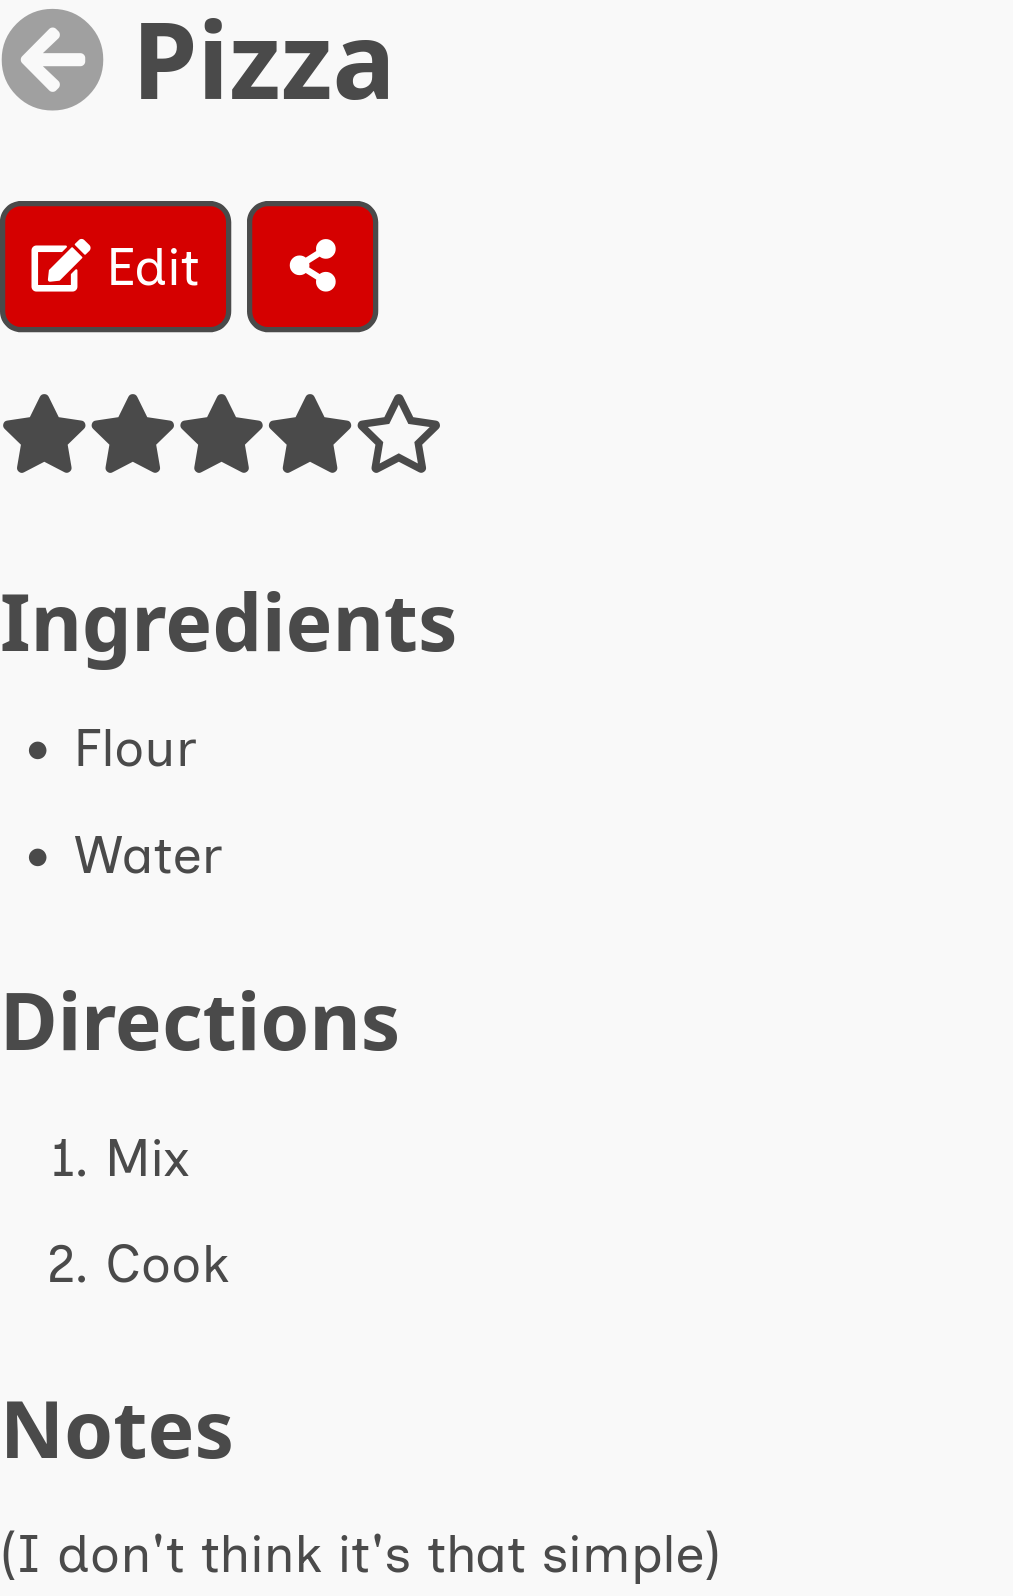
\includegraphics[width=0.45\textwidth]{assets/en/recipe.png}
    \end{figure}

    To edit or delete it, just click on the \emph{Edit} button.

    To ensure a correct formatting, make sure to write the ingredients and the
    directions in multiple lines.

    To hide the stars you can set the stars number to 0.

	\subsection{Sharing}

	If you'd like to share a recipe you can click the \emph{Share} button, and
    you will able to download a pdf, or generate a link (that can be revoked
    anytime), with which anybody can see your recipe. If shared with a link,
    every edit you make will be seen by everyone.

    \begin{figure}[H]
        \centering
        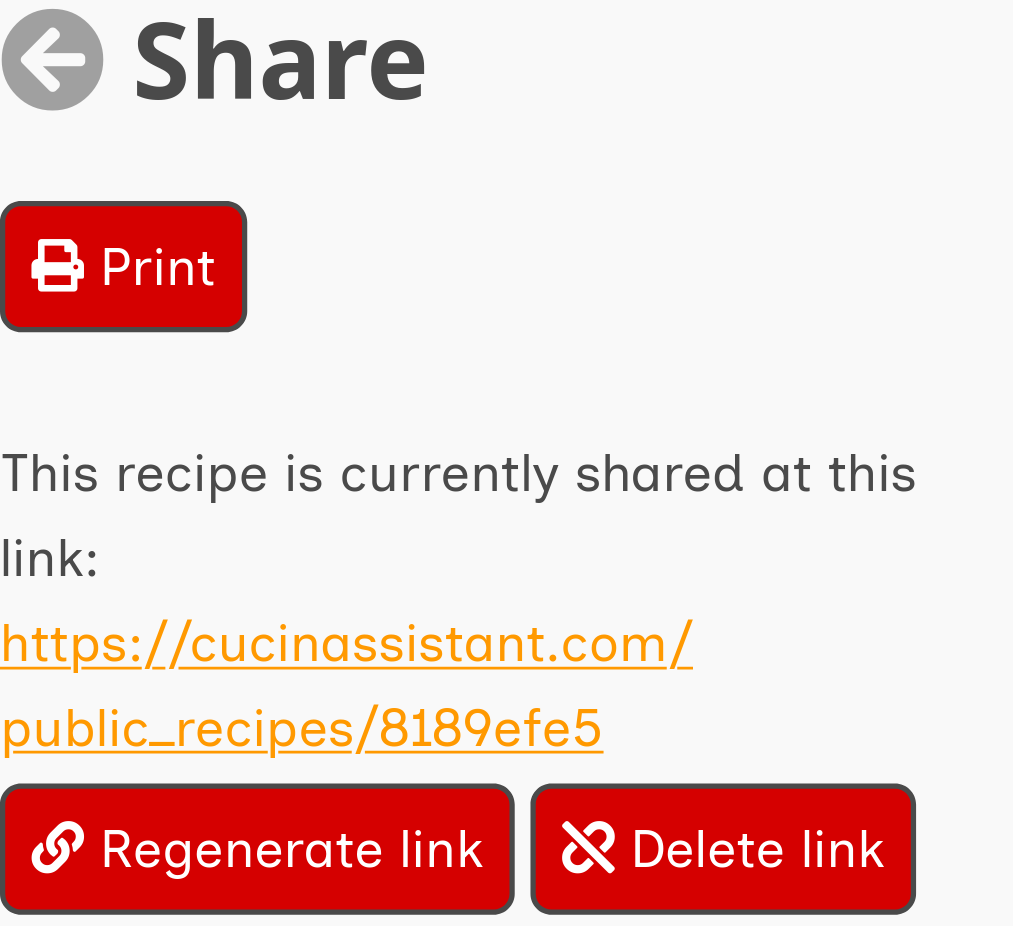
\includegraphics[width=0.45\textwidth]{assets/en/recipe_sharing.png}
    \end{figure}

	Registered users can save a copy of a recipe shared with a link. If they do
    so, the owner's changes won't be forwarded to the copies, but the
	copies will remain even if the original link is revoked.
\end{document}
